\documentclass[../proyecto.tex]{subfiles}

\begin{document}
\chapter{Análisis del problema}
\section{WiFi}

Para poder usar una red Wi-Fi el primer paso que debe realizar un cliente es encontrar la red, para ello debe realizar un proceso de escaneo del medio para encontrar una red a la que unirse. Existen dos métodos de escaneo de redes Wi-Fi: pasivo y activo \cite{ieee80211_2016}. En el escaneo pasivo el cliente enciende el receptor y escanea en cada canal esperando que un punto de acceso se anuncie mediante un \textit{beacon frame}, el cliente almacena en un \textit{buffer} todos los \textit{bacons} recibidos para posteriormente extraer información del punto de acceso que lo emitió, este método no se considera muy eficiente. Para mejorar este proceso de descubrimiento la mayoría de dispositivos suelen utilizar el método de escaneó activo en que el cliente también analiza cada canal uno a uno pero en lugar de esperar a que la red se anuncie realiza un escaneo activo para encontrar la red, para ello envía \textit{Probe Request frames}, normalmente a la dirección broadcast (ff:ff:ff:ff:ff:ff), solicitando respuesta de un punto de acceso pudiendo indicar opcionalmente el identificador de la red (SSID) este último tipo se denomina \textit{directed probe request}, una vez emitido inicia un contador a cero y espera una respuesta, si no la recibe pasa al siguiente canal. El tiempo que espera una estación para recibir una respuesta está definido por cada fabricante pero suele rondar los 10 milisegundos, en cualquier caso, suele ser menor que el intervalo con el que los puntos de acceso emiten los \textit{beacons}.

Cuando un punto de acceso detecta un \textit{Probe Request} con el identificador de su red responde al cliente con un \textit{Probe Response frame}\\
% añadir más información sobre la respuesta del punto de acceso

En el escaneo pasivo la identidad del cliente es anónima mientras que el escaneo activo el cliente envía su dirección MAC que es un identificador único asignado por el fabricante, esto propicia que este método de descubrimiento pueda ser utilizado por terceros para detectar y registrar la presencia dispositivos en punto y tiempo concretos.\\
% contexto de que aporta al proyecto que exista este tipo de escaneo

Las tramas \textit{Probe Request frames} utilizadas en el escaneo activo son un subtipo de las tramas de tipo \textit{Management} definidas en la subcapa MAC (\textit{Medium Access Control}) del estándar IEEE 802.11, este tipo de tramas se utilizan para funciones de supervisión como puede ser unirse o salir de una red.\\

Una trama MAC está compuesta de los siguientes componentes:
\begin{enumerate}
  \item Una cabecera MAC (\textit{MAC header}).
  \item El cuerpo de la trama (\textit{Frame body}) determinado por el tipo y subtipo.
  \item Un FCS (\textit{Frame Check Sequence}) que contiene un CRC de 32 bits.
\end{enumerate}

\begin{figure}[h!]
\centering
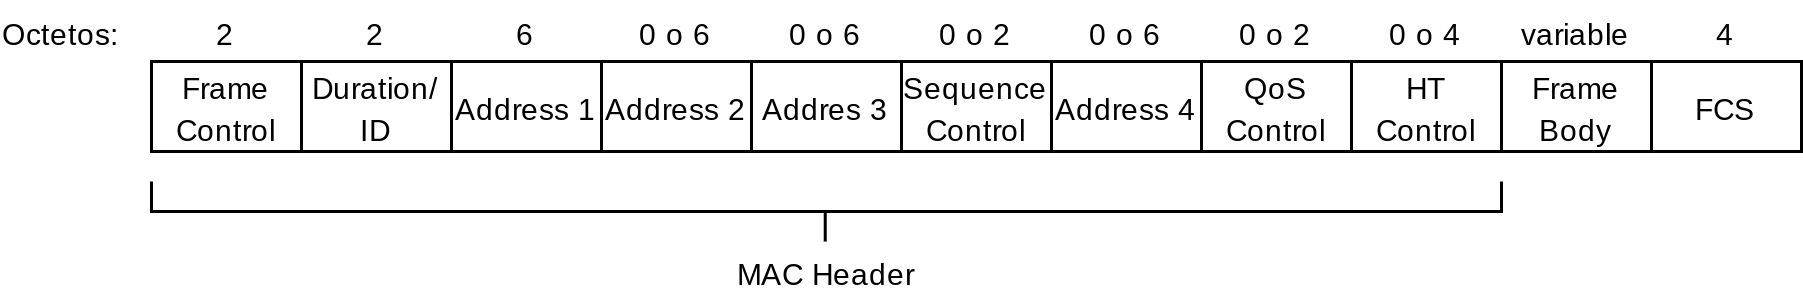
\includegraphics[scale=0.8]{analisis/mac_frame_format}
\caption{IEEE 802.11 MAC frame}
\label{fig:ieee80211_mac_frame}
\end{figure}

Los primeros tres campos (\textit{Frame Control}, \textit{Duration/ID} y \textit{Address 1}) y el último campo (\textit{FCS}) constituyen el conjunto mínimo de campos necesarios y están presentes en todas las tramas. El resto de campos están presentes solo en determinados tipos y subtipos de tramas.\\

Para el propósito de este proyecto solo necesitamos analizar la cabecera de la trama, en concreto los campos más relevantes son el \textit{Frame Control} que permitirá determinar el tipo de trama y el campo \textit{Address 2} que almacenará la dirección MAC de la estación emisora.\\

Existen dos formatos diferentes para el campo \textit{Frame Control}, este formato viene determinado por los campos \textit{Type} y \textit{Subtype}, en este caso es de interés el formato para las tramas cuyo tipo es diferente de 1 o el subtipos es diferente de 6, en cuyo caso el campo \textit{Frame Control} será como el ilustrado en la Figura \ref{fig:ieee80211_frame_control_field}

\begin{figure}[h!]
\centering
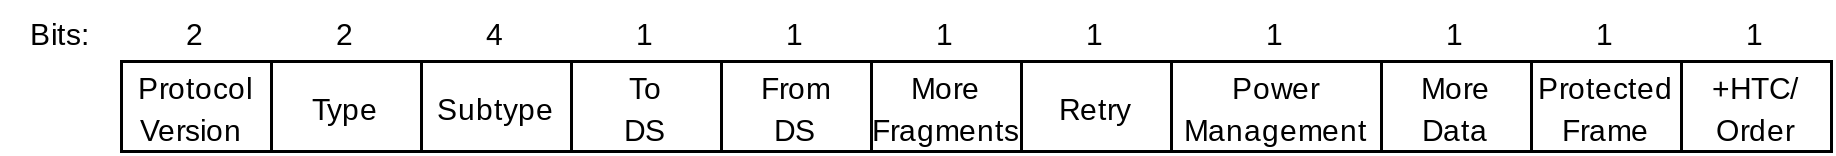
\includegraphics[scale=0.8]{analisis/frame_control_field}
\caption{IEEE 802.11 Frame Control field}
\label{fig:ieee80211_frame_control_field}
\end{figure}

El campo \textit{Type} permite determinar si se trata de una trama de tipo \textit{Management}, en la Tabla \ref{table:tipos_trama} se muestran los posibles valores que puede tomar el campo.\\

\begin{table}[h!]
\centering
\begin{tabular}{ |l|m{20em}| }
\hline
\textbf{Type} & \textbf{Descripción} \\
\hline\hline
00  & Management          \\ \hline
01  & Control  \\ \hline
10  & Data \\ \hline
11 & Extension \\ \hline
\end{tabular}
\caption{Tipos de trama}
\label{table:tipos_trama}
\end{table}

Una vez identificada la trama como tipo \textit{Management} (00) los posibles valores que puede tomar el campo \textit{Subtype} son los mostrados en la tabla \ref{table:subtipos_trama}, en concreto el valor para las tramas del subtipo \textit{Probe Request} es el 0100.

\begin{table}[h!]
\centering
\begin{tabular}{ |l|m{20em}| }
\hline
\textbf{Subtype} & \textbf{Descripción} \\
\hline\hline
0000  & Association Request  \\ \hline
0001  & Association Response \\ \hline
0010  & Reassociation Request \\ \hline
0011  & Reassociation Response \\ \hline
0100  & Probe Request \\ \hline
0101  & Probe Response \\ \hline
0110  & Timing Advertisement \\ \hline
0111  & Reserved \\ \hline
1000  & Beacon \\ \hline
1001  & ATIM \\ \hline
1010  & Disassociation \\ \hline
1011  & Authentication \\ \hline
1100  & Deauthentication \\ \hline
1101  & Action \\ \hline
1110  & Action No Ack \\ \hline
1111  & Reserved \\ \hline
\end{tabular}
\caption{Subtipos de trama para el tipo \textit{Management}}
\label{table:subtipos_trama}
\end{table}

Al identificar una trama de tipo \textit{Management} y subtipo \textit{Probe Request} podemos confirmar que el campo \textit{Address 2} contendrá la dirección de la estación que ha emitido el \textit{Probe Request}.

\section{Bluetooth Low Energy}

\textit{Bluetooth Low Energy} (BLE) es una tecnología de red inalámbrica originalmente diseñada por Nokia bajo el nombre Wibree y adoptada después por el  el \textit{Bluetooth Special Interest Group}, empezó como parte de la especificación Core del Bluetooth 4.0 y fue puesta en el mercado en 2010. Desde el principio el propósito de su desarrollo fue diseñar un estándar de radio con el menor consumo posible, enfocado a dispositivos de bajos coste y con un ancho de banda bajo. A pesar del poco tiempo que lleva en el mercado a tenido una gran adopción debido al gran crecimiento del mercado de dispositivos móviles y \textit{wearables}.\\

% más datos sobre las posibildiades que ofrece BLE

BLE trabaja con 40 canales en la banda ISM de 2.4 GHz cada uno separado por 2MHz y define dos tipos de transmisiones: datos y \textit{advertising}. 37 de estos canales se utilizan para las conexiones de datos y los últimos tres canales (37, 38 y 39) son usados como canales de \textit{advertising} para establecer nuevas conexiones o enviar datos de difusión.

% Tipos de direcciones

BLE solo tiene un formato de paquete y dos tipos de paquetes: datos y \textit{advertising}. Un paquete de \textit{advertising} está compuesto de una cabecera, que incluye entre otros datos la dirección bluetooth del dispositivo emisor, y una carga útil de datos de hasta 31 bytes. Estos paquetes se emiten por \textit{broadcast} a un ratio de entre 20 ms y 10.24 s.

% explicación de interval y windows en el scaner



\section{ESP8266}

El ESP8266, oficialmente ESP8266EX, es un SoC WiFi de bajo coste con una pila TCP/IP completa producido por Espressif Systems, una compañía China con sede en Shangai enfocada en el desarrollo de soluciones IoT. \cite{esp8266_overview} \\

\subsection{SoC ESP8266EX}
Espressif desarrollo este SoC pensando en las necesidades de la industria del Internet of Things, como son el bajo consumo energético, un diseño compacto y la fiabilidad y durabilidad. Con una capacidad WiFI completa y autónoma puede funcionar de forma independiente o como adaptador WiFi para cualquier controlador a través de las interfaces SPI/SDIO o UART. Estas cualidades han propiciado que su utilización se haya extendido en la industria de la domótica, por ejemplo, en enchufes y bombillas inteligentes. \\

Integra un microcontrolador Tensilica L106 de 32 bits (RISC) de bajo consumo que trabaja a unos 80 MHz por defecto pudiendo alcanzar hasta 160 MHz. Además incorpora otros componentes de interfaz como SDIO, SPI, I2C, I2S, UART, PWM, conversor ADC de 10 bits y 17 GPIO. Todos estos componentes se encuentran empaquetados en tan solo 5 mm x 5 mm en un formato QFN de 32 pines (Figura \ref{fig:esp8266_soc_pinout}). En el SoC no viene incluida la memoria ROM, debe utilizarse una flash externa por SPI y soporta hasta 16 MB. \cite{esp8266_datasheet}\\


\begin{figure}[h!]
\centering
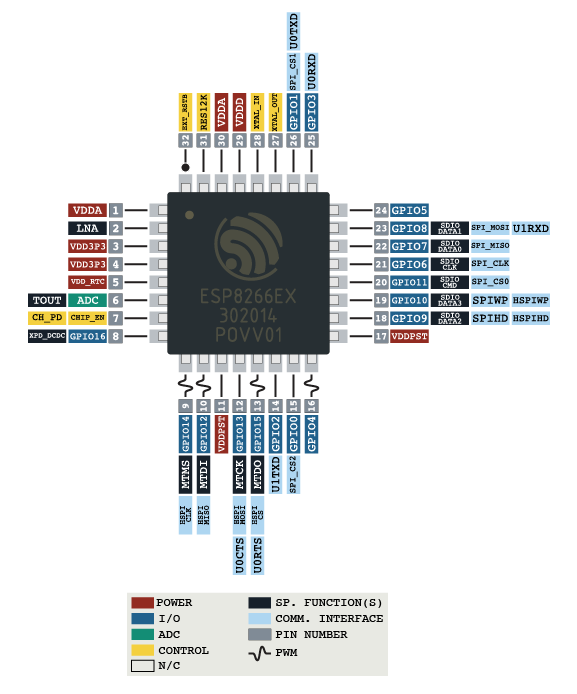
\includegraphics[scale=0.5]{analisis/esp8266_soc_pinout}
\caption{ESP8266EX SoC Pinout}
\label{fig:esp8266_soc_pinout}
\end{figure}

\begin{center}
\begin{tabular}{ |l|m{20em}| }
\hline
Voltaje de operación      & 2.5V $\sim$ 3.6V          \\ \hline
Consumo                   & 20 uA - 170 mA (80 avg.)  \\ \hline
Temperatura de operación  & -40°C $\sim$ 125°C        \\ \hline
Procesador                & Tensilica L106 32-bit     \\ \hline
Frecuencia de reloj       & 80 MHz / 160 MHz          \\ \hline
Interfaces                & UART, SDIO, SPI, I2C, I2S, IR Remote Control, GPIO, ADC y PWM                           \\ \hline
GPIO pins                 & 17                        \\ \hline
RAM (espacio de usuario)  & < 50 kB                     \\ \hline
Protocolos WiFi           & 802.11 b/g/n (HT20)       \\ \hline
Rango de frecuencias WiFi & 2.4G $\sim$ 2.5G (2400M $\sim$ 483.5M) \\ \hline
\end{tabular}
\end{center}


\subsection{Módulos}

Debido a que el ESP8266 viene en un pequeño empaquetado (QFN-21) algunos fabricantes han desarrollado módulos (MCU) que facilitan su uso, proporcionando componentes necesarios para el desarrollo como son la memoria flash externa y pines externos para GPIO.\\

\subsubsection{ESP-WROOM-02}

Espressif dispone de sus propio módulos, la serie ESP-WROOM-02 \cite{espwroom02_overview}, el módulo base \cite{espwroom02_datasheet} lleva el mismo nombre que la serie y tiene un tamaño de 18 mm x 20 mm e integran una memoria flash SPI de 2 MB y una antena PCB, además dispone de 18 pines (Figura \ref{fig:esp01_pinout}).\\

\begin{figure}[h]
\centering
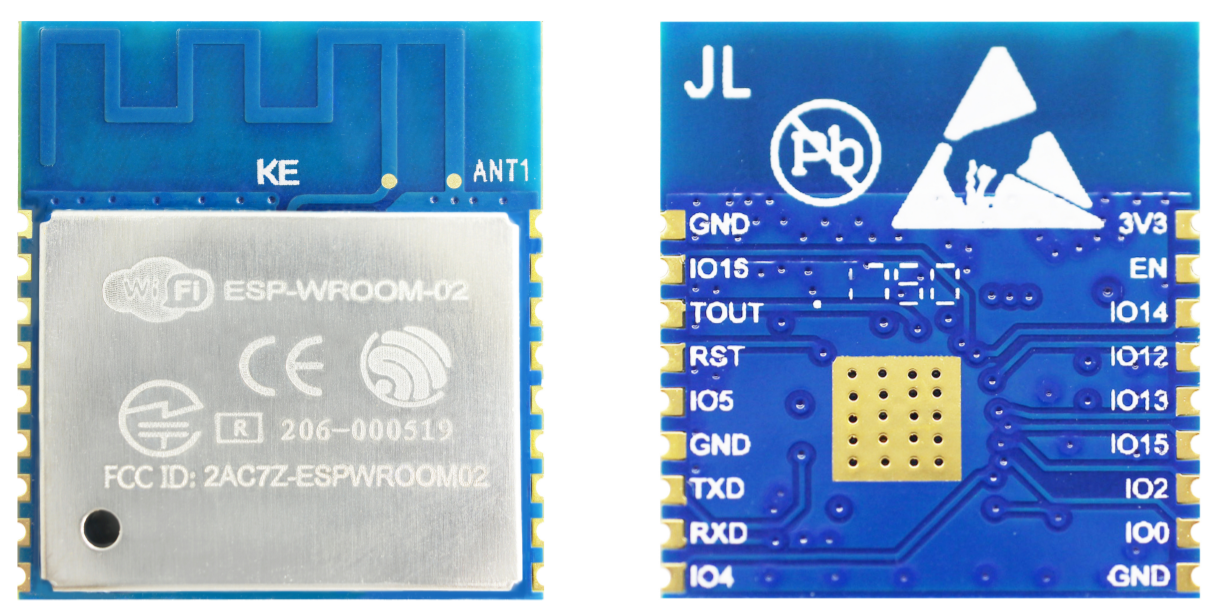
\includegraphics[scale=0.2]{analisis/esp_wroom_02}
\caption{Módulo ESP-WROOM-02}
\label{fig:esp_wrom_02}
\end{figure}

Existen otros tres modelos: ESP-WROOM-02S, ESP-WROOM-02D y ESP-WROOM-02U. El ESP-WROOM-02S \cite{espwrooms2_datasheet} es una pequeña revisión del modelo base con un rediseño de la placa (16 mm × 23 mm). Los módulos ESP-WROOM-02D y ESP-WROOM-02U  \cite{espwroom02d_02u} cuentan con un mejor rendimiento en el apartado de radiofrecuencia y además de las versiones de 2 MB de memoria flash cuentan con una variante de 4 MB, además el modelo ESP-WROOM-02U prescinde de la antena PCB a cambio de un conector IPEX para una anterna externa, viéndose reducido el tamaño del módulo a 18 mm x 14.3 mm.\\

\subsubsection{ESP-XX}

A pesar de que el fabricante original del ESP8266, Espressif, dispone de sus propios módulos, este SoC empezó realmente a popularizarse en el 2014 con el módulo ESP-01 creado por un tercer fabricante, Ai-Thinker. El módulo añade una memoria flash externa QSPI, una antena impresa en la PCB y proporciona salida para algunos de los pines del ESP8266 (Figura \ref{fig:esp01_pinout}).\\

\begin{figure}[h]
\centering
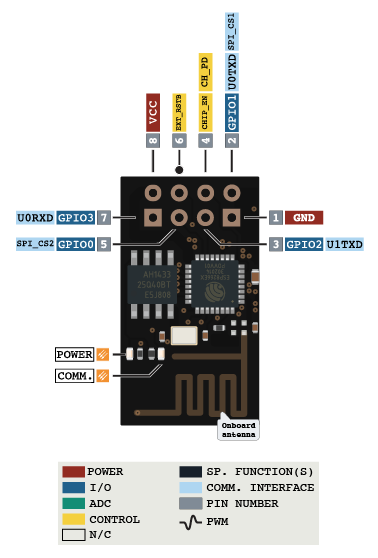
\includegraphics[scale=0.5]{analisis/esp01_pinout}
\caption{ESP-01 Pinout}
\label{fig:esp01_pinout}
\end{figure}

Desde este primer modelo se han desarrollado multitud de modelos con variaciones respecto al número de pines expuestos, tipo de antena y memoria flash; pero manteniendo el mismo SoC ESP8266EX. Se les conoce como módulos ESP-XX y la última versión es el ESP-14 que combina en el mismo encapsulado el SoC ESP8266EX junto con un microcontrolador STMicro STMS003F3P6. Aunque el modelo más utilizado de esta serie es el ESP-12 y sus variantes con apantallamiento y un mayor número de conexiones, en concreto 22, a excepción del módulo ESP-12S que cuenta con 16. (Figura \ref{fig:esp12e_pinout}).\\

\begin{figure}[H]
\centering
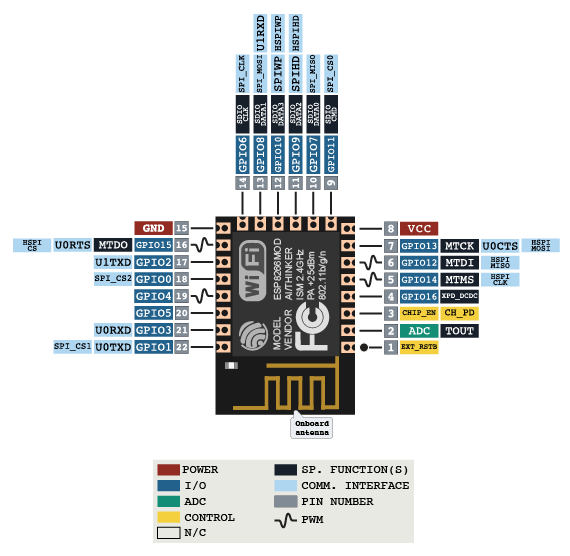
\includegraphics[scale=0.5]{analisis/esp12e_pinout}
\caption{ESP-12E Pinout}
\label{fig:esp12e_pinout}
\end{figure}

Aunque estos módulos son más cómodos seguimos teniendo la necesidad de adquirir un adaptador USB-Serial y un regulador de voltaje y cablearlos al módulo para poder programarlo.\\

\subsection{Módulos de desarrollo}

Estos módulos están enfocados al desarrollo y a facilitar la creación de prototipos. Para facilitar el desarrollo incluyen un puente USB-Serial integrado en la placa y un conector micro-USB junto con un regulador de voltaje para proporcionar energía a la placa y conectividad con el ordenador.\\

Algunos modelos están basado en módulos ESP-XX de Espressif como el Adafruit Feather HUZZAH \cite{adafruit_feather_huzzah} que utiliza un módulo Ai-Thinker ESP-12S, en la figura \ref{fig:adafruit_feather_huzzah_pinout_2} se pude apreciar como el módulo de Ai-thinker está soldado directamente encima de la placa de desarrollo.\\~\\

\begin{figure}[H]
\centering
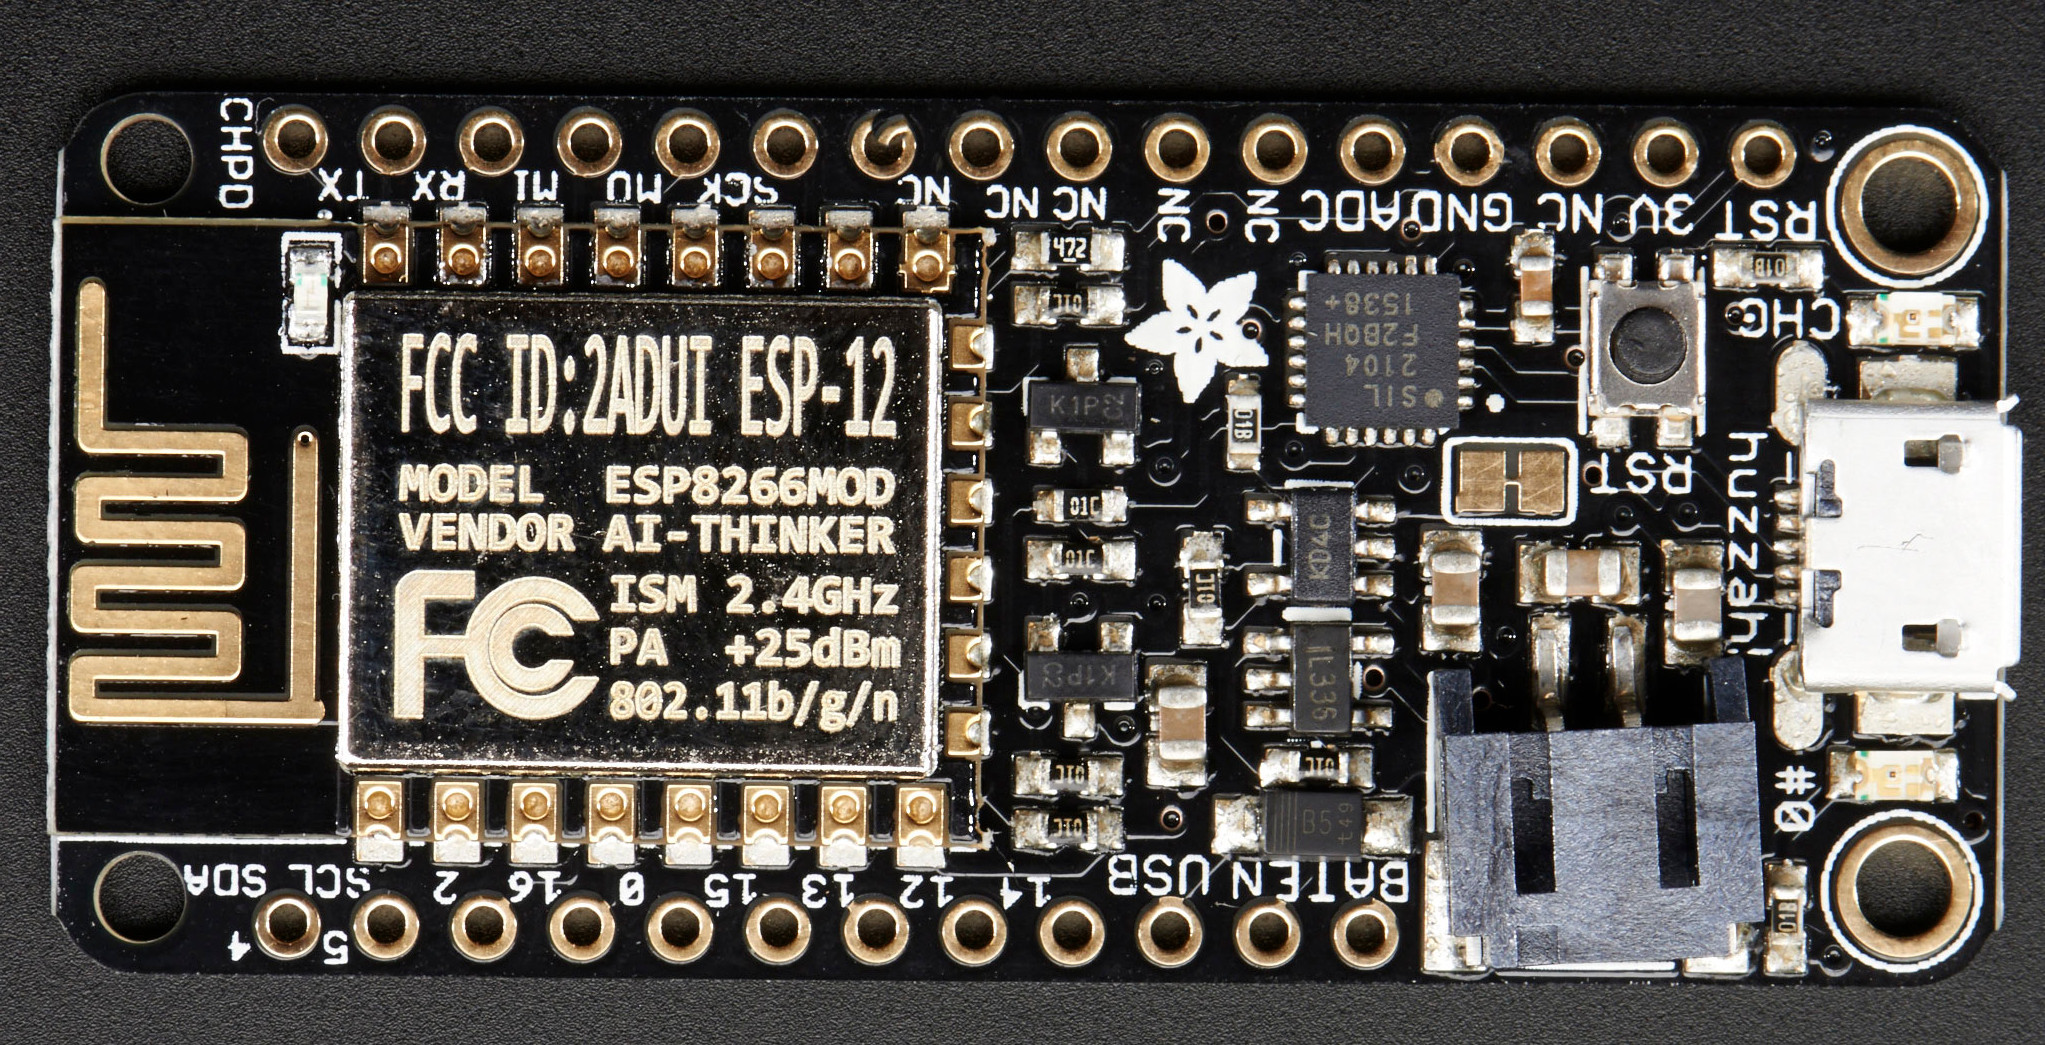
\includegraphics[scale=0.12]{analisis/adafruit_feather_huzzah_pinout_2}
\caption{Adafruit Feather HUZZAH}
\label{fig:adafruit_feather_huzzah_pinout_2}
\end{figure}

Otros módulos de desarrollo no usan un módulo intermediario, en su lugar incorporan directamente el chip en la placa como es el caso del WEMOS D1 Mini Pro \cite{wemos_d1_mini_pro} que utiliza un ESP8266EX (Figura \ref{fig:wemos_d1_mini_pro}).\\

\begin{figure}[h]
\centering
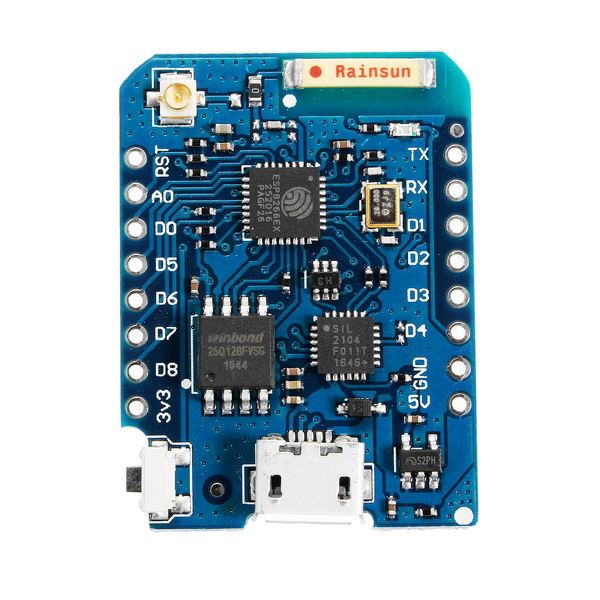
\includegraphics[scale=0.5]{analisis/wemos_d1_mini_pro}
\caption{WEMOS D1 Mini Pro}
\label{fig:wemos_d1_mini_pro}
%https://wiki.wemos.cc/products:retired:d1_mini_pro_v1.1.0
\end{figure}

\subsubsection{NodeMCU}
NodeMCU es un hardware libre basado en el módulo ESP-12, fue diseñado y liberado por la empresa Altium Designer \cite{nodemcu_devkit_repository}, este módulo surgió tras la creación del firmware libre homónimo basado en el lenguaje Lua. Esta placa incluye un puente USB-Serial, un conversor de voltaje  a través de un micro-USB y además dispone de un LED y botón de reset integrados. Al ser un diseño libre existen varias empresas que comercializan este módulo de desarrollo, las más conocidas Lolin y Amica.\\



La primera versión en popularizarse fue la denominada v1.0/v2 de Amica (Figura \ref{fig:nodemcu_v2_devboard_pinout}) que utiliza un ESP-12E por lo que tiene más pines que el modelo original, dispone de una memoria flash de 4 MB, antena PCB y además es más estrecha (48mm x 26 mm) por lo que facilita su uso en una breadboard. Esta placa tuvo gran acogida en la comunidad de NodeMCU y es considerada la versión oficial aunque esto no tenga mucho sentido siendo un diseño de hardware libre, otros fabricantes como Lolin terminaron fabricando esta versión.\\

\begin{figure}[h]
\centering
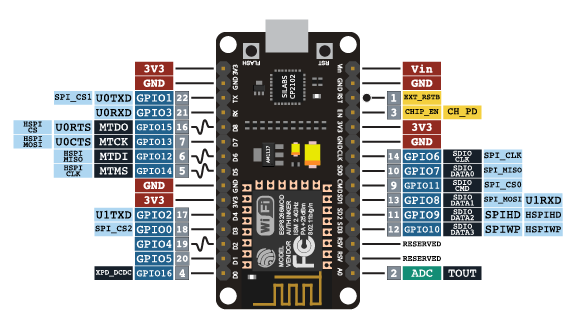
\includegraphics[scale=0.4]{analisis/nodemcu_v2_devboard_pinout}
\caption{NodeMCU v1.0/v2 Amica}
\label{fig:nodemcu_v2_devboard_pinout}
\end{figure}

La versión más comercializada actualmente es la v1.0/v3 creada por la empresa Lolin, incorpora pocos cambios, cambiaron el conversor serial CP2102 por un CH340G y reusaron dos de los pines reservados en la v2 para sacar un GND y un VUSB. Como desventaja el tamaño se incrementó (58 mm x  31 mm) dificultando su uso en una breadboard.\\

Ambos modelos podemos encontrarlos por un precio de entre 4 € y 8 € dependiendo del volumen de compra.\\

\subsection{Adafruit Feather HUZZAH}

Feather \cite{adafruit_feather_huzzah} es una placa de la empresa Adafruit Industries, tiene unas dimensiones de 51 mm x 23 mm, incorpora un chip USB-Serial SiLabs CP2104 que permite cargar el código en la placa a una velocidad de 921600 baudios, una memoria flash de 4 MB, una antena PCB y como elemento diferenciador de otras placas incluye un conector para baterías de polímero de litio de 3.7 V (Figura \ref{fig:adafruit_feather_huzzah_pinout}) que puede ser cargada a través de la conexión micro-USB. Se puede adquirir por entre 12 € y 15 €.

\begin{figure}[H]
\centering
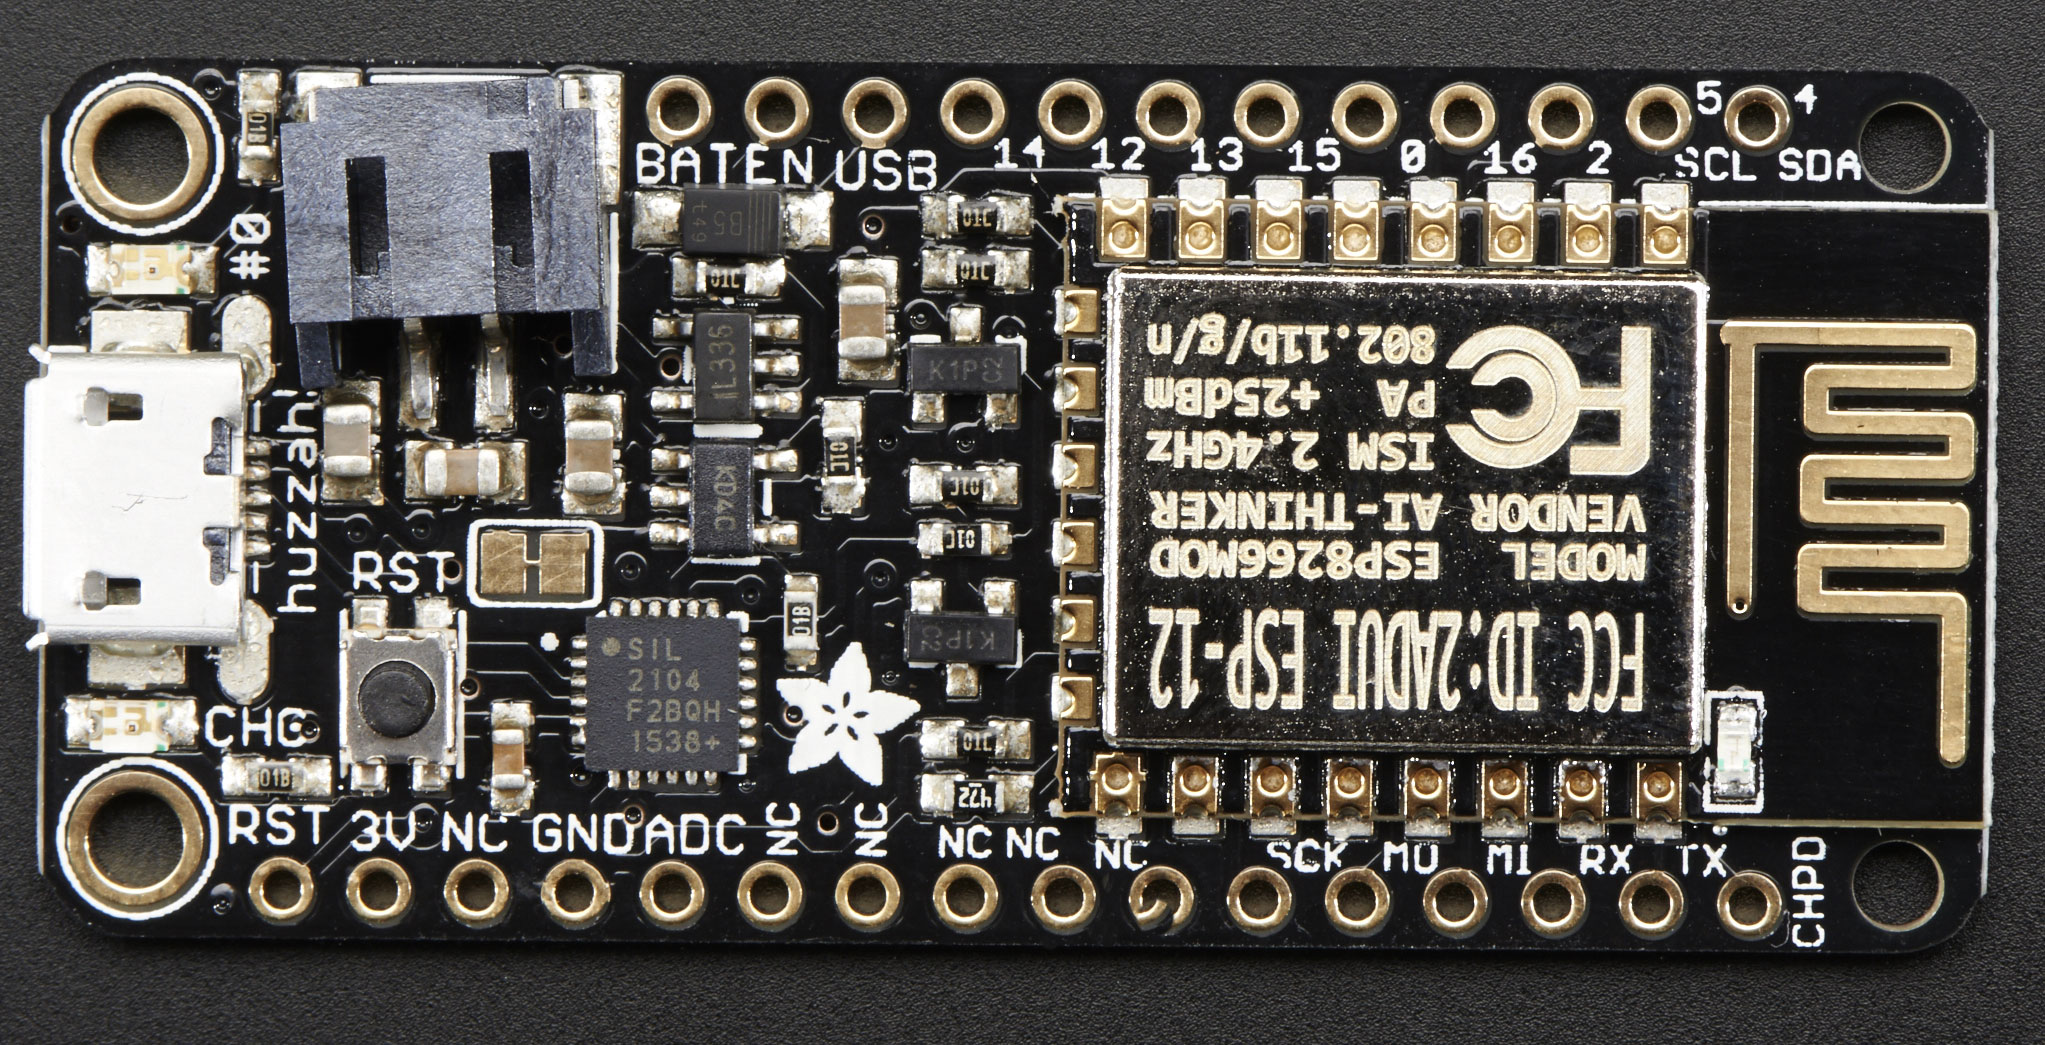
\includegraphics[scale=0.2]{analisis/adafruit_feather_huzzah_pinout}
\caption{Adafruit Feather HUZZAH Pinout}
\label{fig:adafruit_feather_huzzah_pinout}
\end{figure}

\subsubsection{SparkFun ESP8266 Thing}
ESP8266 Thing \cite{sparkfun_thing_official_page} es una placa de la empresa SparkFun Electronics, tiene un tamaño de 55 mm x 26 mm, utiliza directamente un SoC ESP8266EX e incorpora un chip USB-Serial FT231XS con un conector micro-USB, una memoria flash de 4 MB, una antena PCB y la un conector
\begin{figure}[H]
\centering
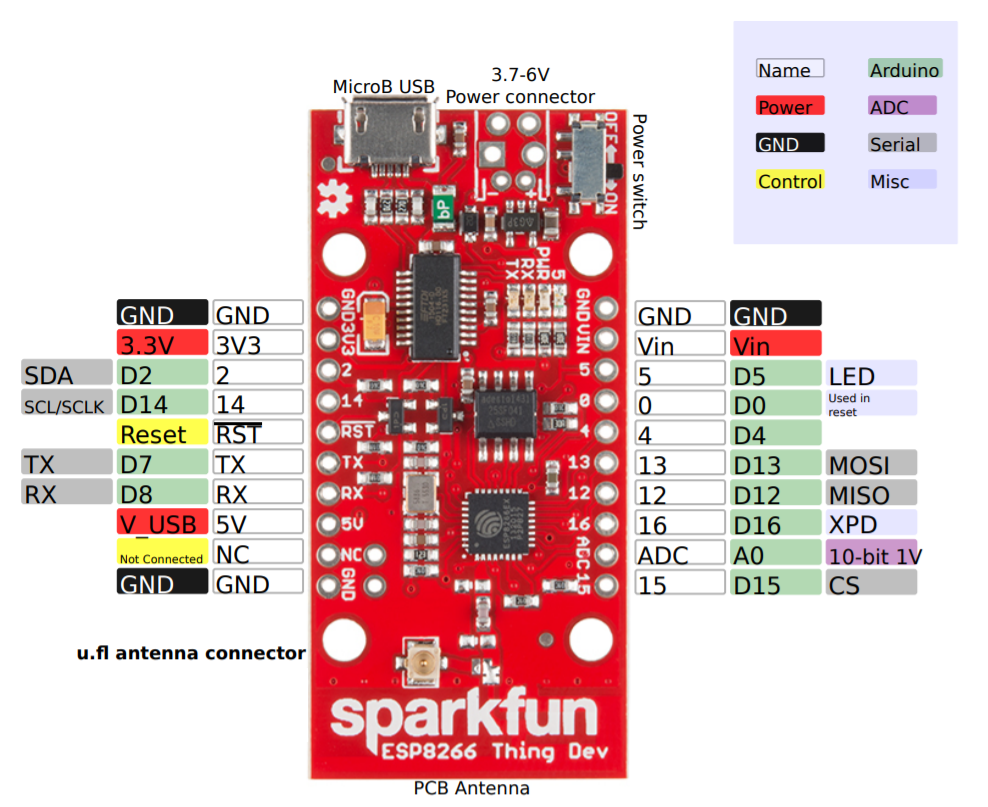
\includegraphics[scale=0.25]{analisis/sparkfun_thing_pinout}
\caption{SparkFun ESP8266 Thing Pinout}
\label{fig:sparkfun_thing_pinout}
\end{figure}


\subsubsection{Elección}

Para el desarrollo de este proyecto se ha elegido el módulo de desarrollo WEMOS D1 Mini Pro, con unas dimensiones de 34.2 mm x 25.6 mm y un peso de 3 g es una de las placas más pequeñas del mercado, con un tamaño ligeramente más grande que un módulo ESP-12 (24.0 mm × 16.0 mm) incorpora un conversor P2104 USB-TO-UART, antena cerámica incorporada memoria flash de 16 MB y un regulador de tensión que permite alimentarlo a 5 V a través de un micro-USB. Una de los principales motivos para la elección de este módulo de desarollo es la posibilidad de conectar una antena externa para mejorar el alcance mediante un conector de tipo U.FL. \\

Otra de las ventajas de este módulo de desarrollo, a pesar de estar fuera del alcance de este proyecto, es la posibilidad de ampliar la funcionalidad a través de la conexión de expansiones en formato shields. Existe una gran variedad shields como, por ejemplo, pantalla oled, relé o controlador de motores (Figura \ref{fig:wemos_d1_mini_shields}).\\

\begin{figure}[h]
\centering
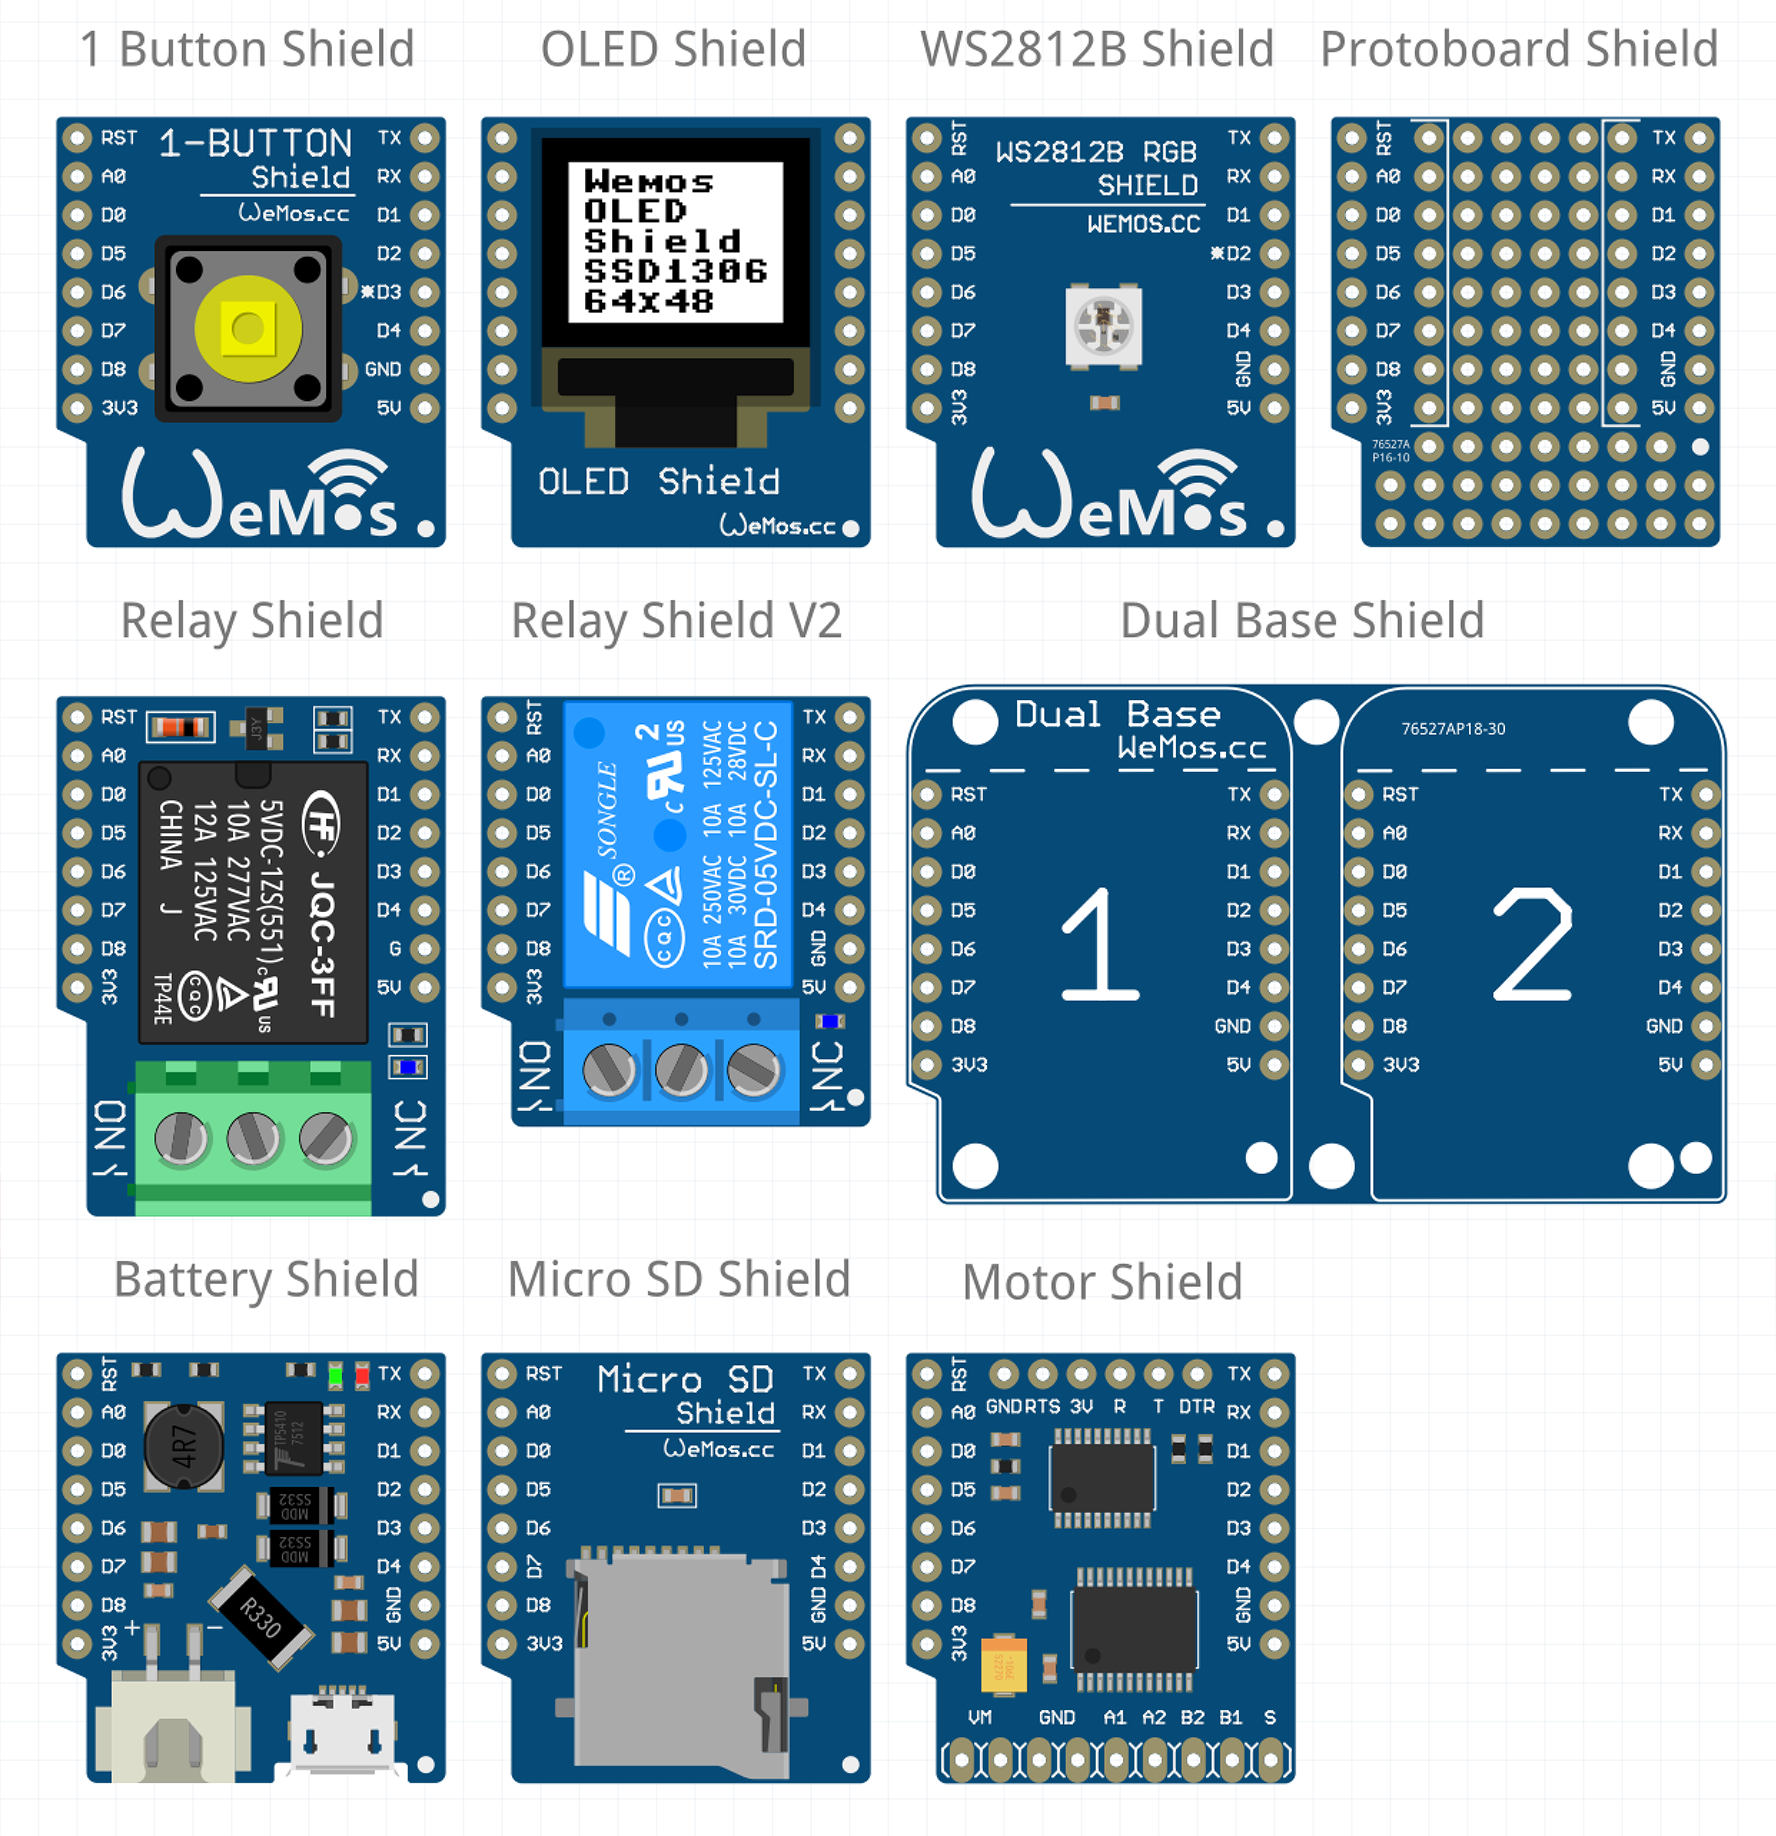
\includegraphics[scale=0.15]{analisis/wemos_d1_mini_shields}
\caption{WEMOS D1 Mini Shields}
\label{fig:wemos_d1_mini_shields}
%https://github.com/mcauser/Fritzing-Part-WeMos-D1-mini-Shields
\end{figure}

Como desventaja cabría comentar que tiene un menor número de pines disponibles respecto a otros módulos de desarrollo, aunque para el ámbito de este proyecto no supone un problema.\\





Respecto al lenguaje utilizado para desarrollar en estos módulos, en sus inicios algunos módulos fueron creados para trabajar con ciertos lenguajes o IDEs, un ejemplo es es el módulo NodeMCU \cite{nodemcu_official_page} y el lenguaje Lua, actualmente es posible usar la mayoría de lenguajes.
% [1]https://www.espressif.com/en/products/hardware/esp8266ex/overview
% [2]https://www.espressif.com/sites/default/files/documentation/0a-esp8266ex_datasheet_en.pdf
% [3]https://www.espressif.com/en/products/hardware/esp-wroom-02/overview


% FIGURAS
% [1] https://raw.githubusercontent.com/acrobotic/Ai_Docs/master/pinouts/esp8266_soc/esp8266_soc-01.png
% [2] ESP-01 Pinout https://github.com/acrobotic/Ai_Docs/blob/master/pinouts/esp8266_esp01/esp8266_esp01-01.png
\end{document}
